%
% Tutorial -- Power Amplifier Design
%
% Copyright (C) 2005 Thierry Scordilis <thierry.scordilis@free.fr>
%
% Permission is granted to copy, distribute and/or modify this document
% under the terms of the GNU Free Documentation License, Version 1.1
% or any later version published by the Free Software Foundation.
%

\section*{warning}

\textit{
This chapter will describe an RF design issue using QUCS. The author assume that the basic manipulation of qucs is known. You will find herein mainly a MacOsX description that is close to a linux or unices architecture.
}

\tutsection{Field of interest}

This power amplifier will be used in a more complex system taht I can not describe herein, but the application is inside the $868MHz$ ISM frequency band. This amplifier is considered as power amplifier since it is not a LNA, but its power is not very high as well as you can see in the following system specification. It is more a low input power amplifier driving relatively low current. An application note with really high power level such several watts will be an other chapter.

%-------------------------------------------------------------------------

\tutsection{System consideration}

As a system point of view we need first to specify what kind of function we need. this function will be defined as mentionned in table \ref{design:pa:systemSpecification}.


\begin{table}[htp]
\caption{System specification for the design of a PA}
\begin{center}
\begin{tabular}{|c|c|c|c|c|c|} \hline
parameter & description 					& min   & typ     & max   & unit \\ \hline \hline
$F_o$     & frequency of operation		& $863$ & $868.6$ & $870$ & MHz \\
$Icc$ 	   & current consumption        &       & $20$    & $25$    & mA \\ \hline
$Z_{in}$  & input impedance            &       & $50$    &        & $\Omega$ \\
$Z_{out}$  & output impedance            &       & $50$    &        & $\Omega$ \\ \hline
$P_{in}$   & input power                &   $-15$ & $-10$ & $-8$ & dBm \\
$P_{out}$   & input power                &   $5$ & $10$ & $12$ & dBm \\ \hline
$V_{cc}$   & DC supply voltage                &   $2.45$ & $2.5$ & $2.55$ & V \\ \hline
\end{tabular}
\end{center}
\label{design:pa:systemSpecification}
\end{table}

Cost issue is very important, therefore only one active component is allowed, and the BOM \footnote{Bill Of Material} should be reduced as much as possible.

\bigskip

This design should work on a FR4 PCB used in a production line. The parameters of such substrate is quite uncontrolled but can be caracterized, as long as you keep the same supplier ( avoid strange suppliers who can change the FR4 composition without notice ).

As mentionned previously you can describe a substrate inside the library with the following lines :

\begin{verbatim}
<SUBST FR4_ 1 0 0 -30 24 0 0 
	"4.7" 1 "0.7 mm" 1 "35 um" 1 "2e-4" 1 "0.022e-6" 1 "0.15e-6" 1
	>
\end{verbatim}

The height of the substrate is $0.7$mm but this describe only one RF layer of the full implementation of the circuit which is a four layour board. The two inner layer are power and ground, the top and bottom layer are RF layers.


\tutsection{Biasing consideration}

In this section we will see how the biasing is made, especially using a emitter feed back technic. If you remember well the data sheet of the transistor, there is a huge dispersion on the $h_{FE}$, and some other dispersion have to be taken into account : resistance, supply voltage, \ldots.

\begin{figure}[htbp]
\begin{center}
	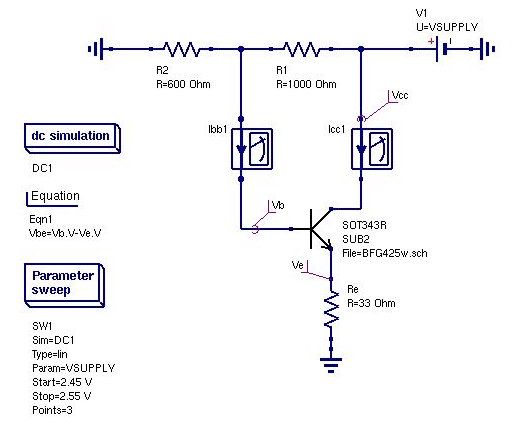
\includegraphics[scale=0.7]{biasSchem}
	\caption{Schematics used for this study}
	\label{design:pa:bias:schema}
\end{center}
\end{figure}

The used schematics is shown is fig \ref{design:pa:bias:schema}. But we need to evaluate the component first. Using small calculus it is easy to figure out the different resistance :

assuming that 

\begin{equation}
I_c = \beta I_b 
\end{equation}

\begin{equation}
I_{biasBridge} \ll I_b
\end{equation}

\begin{equation}
I_{biasBridge} = \frac{I_c}{10}
\end{equation}

\begin{equation}
R_e = \frac{V_{cc} - V_{ce}}{I_c}
\end{equation}


\begin{equation}
R_1 + R_2 = \frac{10 \times V_{cc}}{I_c}
\end{equation}

\begin{equation}
R_2 = \frac{10}{I_c} \times ( V_{cc} - V_{ce} + V_{be} )
\end{equation}


The inputs are :
\begin{itemize}
\item $V_{cc} = 2.5 V$
\item $V_{be} = 0.412 V$
\item $I_c = 15 mA$
\end{itemize}

the results are :
\begin{itemize}
\item $R_1 = 1 K\Omega$
\item $R_2 = 600 \Omega$
\item $R_e = 33 \Omega$
\end{itemize}

Using these values on the schematics, we can now see the stability of the design. Adding the fact that the voltage regulator used in this case has an ondulation of 5 mV in the working domain.  You need to simulate the DC schematics by modifying the BF parameter of the transistor from 50 to 120 ( since this feature is not enabled in the current version of Qucs $0.0.7$ ).


\begin{table}[htp]
\caption{Variation of $I_c$ in mA, due to the $V_{cc}$ and $\beta$}
\begin{center}
\begin{tabular}{|c|c|c|c|} \hline
Vcc  vs $\beta$ & 50 & 80 & 120 \\ \hline
2.45	&	12.21	&	13.34	&	14.07	\\
2.50	&	12.62	&	13.78	&	14.54	\\
2.55 	&	13.03	&	14.23	&	15.01	\\ \hline
\end{tabular}
\end{center}
\label{design:pa:bias:variation}
\end{table}

From this table we can extract some stability factor :

\begin{equation}
\frac{\Delta I_{cc}}{\Delta V}\vert _{\beta = 80} = 8.9 \mu A / mV
\end{equation}

\begin{equation}
\frac{\Delta I_{cc}}{\Delta \beta}\vert _{V_{cc} = 2.5} = 30 \mu A
\end{equation}

\begin{equation}
\frac{\Delta I_{cc}}{\Delta T}\vert _{\beta = see note, V_{cc} = 2.5 } = \ldots \mu A / C
\end{equation}

\textbf{Note} : For the temperature dependance, we need to take the minimum $\beta$ for the minimum temperature, and the maximum $\beta$ for the maximum temperature.





\tutsection{Why thermal design ?}

The objective of the thermal design in electronic equipment is to
provide as low a temperature rise, $\Delta$T, above ambiant as is
practical for a product's electronic components.

As a practical matter, a small 3C to 5C component
temperature rise is almost unavoidable, and actually has been found
to be desirable. If the rise is less than that, there can be more
moistrure-related problems, particularly corrosion and electrical
leakage currents.

\begin{itemize}
	\item Improves performance : avoids calibration drift, maintains
	phase lock loops, stabilizes gain, ...

	\item Improves reliability : failure mechanisms accelerate
	rapidly at higher temperatures through metal migration, increased
	ion mobility, ...

	In most electronic components, the failure rate doubles for a
	10C to 15C rise in temperature and the slope is
	exponential ! temperature cycling is even worse.

	Temperature rise is particularly hard on components which depend
	on an internal liquid, such as electrolytic capacitor,
	batteries, and lubricated bearings.

	Sophisticated thermal design is becoming a necessity as devices
	becomes smaller and poxer density increase. Examples : VLSICs and
	surface mount technology SMT.

	\item Improves life : higher $\Delta$T increases mechanical
	stress, failures of connections, metalisation contacts,...
\end{itemize}

\tutsubsection{Thermal management}

The objective of thermal management is to design the internal
thermal environment of the electronic equipment so the equipment
performance will meet customer expectations. Within the range of
environmental conditions where the equipment is expected to operate,
the equipment should perform within specifications and operate
reliably. In general, the designer has little control over the
external environment, so he must design for an anticipated range. He
does have more control over the internal environment, but his
attention should be directed toward the ultimate goal ; maintaining
a suitable environment for the critical components.

Analysis of the thermal environment can usually be divided into
several distinct parts because of almost--isothermal boundaries.
Consider the typical enclosure system, the isothermal boundaries are
:

\begin{itemize}

\item the enclosure at $T_e$
\item the interior at $T_b$
\item the component at $T_c$

\end{itemize}

Because of these boundaries, $\Delta T_{jc}$, $\Delta T_{ca}$ and
$\Delta T_{ja}$ can be solved independently. $\Delta T_{ae}$ and
$\Delta T_{e\infty}$ can also be solved independently for a sealed
enclosure, but are inter--dependent for a vented or forced air
cooled enclosure.

\paragraph{approching the problem}

During the definition stage of a product, the choice of enclosure is
sometimes dictated by a competitor, the customer, or marketing.
Frequently the choice is "as small as possible", thus unwittingly
passing judgment on a particular choice, it is possible to make a
thermal analysis of the proposed enclosure. If the environment
created for the component is unsuitable, then additional cooling
mechanisms must be developped.

One approch is to simplify the problem to one dimensionnal analysis.
Heat energy sources azre assumed to be evenly distributed throughout
the volume. The enclosure surface is assumed to be isothermal. The
enclosure is assuemd to made of a perfect thermal conductor. (
unfortunately, enclosures are more and more being made of plastic, a
thermal insulator, which complicates this sample approch).

The external environment is considered to be the walls of a large
room of surface emissivity , $\epsilon$ , of 1.0 at the same
temperature, $T_\infty$, as the surrounding air, and is capable of
absorbing an infinite amount of heat energy.

Heat transfert by conduction, radiation, free convection, venting,
and forced convection are basically representated by the equation :

\begin{equation}
Q_t = Q_k + Q_r + Q_c + Q_v + Q_f
\end{equation}

The most elusive component, thermal resistance $\Theta_x$, can vary
from simple to very complex. Fortunately, most electronic enclosures
do not have more than three cooling paths and in many cases, the
third path is minor one that can be neglected for ease of
calculation.

The following are some generally accepted guidelines that can be
used to quickly evaluate a design or configuration. These were
obtained from notes provided by \cite{spinelli}.

Maximum power density :

\begin{itemize}

\item
for small painted uniformly heated sealed enclosure
	\begin{itemize}
	\item naturally cooled $< 4 mW/cm^3$
	\item taller than $60 cm < 2 mW/cm^3$
	\end{itemize}

\item
for naturally cooled printed circuit boards $< 16 mW/cm^2$

\item
for forced air cooled printed circuit board $< 110 mW/cm^2$

\item
for small ( $60cm$ or less ) induced draft cooled enclosure $< 20 mW/cm^3$

\end{itemize}

forced air velocities :

\begin{itemize}
\item for PCB cages $> 4 m/sec$
\item for enclosures $< 7.6 m/sec$
\end{itemize}

\tutsection{DC Power dissipation}

An important issue in power amplifier design is the power dissipation. Even if in this particular case the power dissipation is not that obvious, it is nice to see how we can handle this anyway.

\bigskip

As a student you always learn that you can apply kirchoff law on temperature. This only thing you have to know is the correspondance : 

\begin{description}
\item[The temperature : ] is equivalent to the voltage
\item[The power : ] is equivalent to the current 
\item[The thermal resistance : ] is equivalent to the resistance
\end{description}

You can also take into account some calorific capacity, and perturbation from near effect due to the presence of other source of heating, in a dynamic design, but we will only see the DC power dissipation here \ldots from this start point you can then imagine whatever you want.

\bigskip

In order to proceed, we need to create a model for this power dissipation. This model can be very simple on its comprehension but very complex since all the parameters are not well known. Therefore we will need to reduce the level of modelisation that is used.

Here are the input parameters :
\begin{itemize}
\item The DC power dissipation is $15 mA \times 2.5 Volts = 37.5 mW $
\item the thermal resistance of the device is $\theta_{junction_solder}=350 degC/W$
\item the thermal resistance of the ambiante is $\theta th_{pcb_air}=22 degC/W$
\item the ambiante temperature varies from $-25 degC$ to $75 degC$ and $25 degC$ typical
\end{itemize}


The schematics used for this simulation is shown is figure \ref{design:pa:bias:DCpower}\footnote{Note the possiblity to place the results of the simulation directly on the schematics, and some comments on the schematics such as document name, revision, and so on.}.

\begin{figure}[htbp]
\begin{center}
	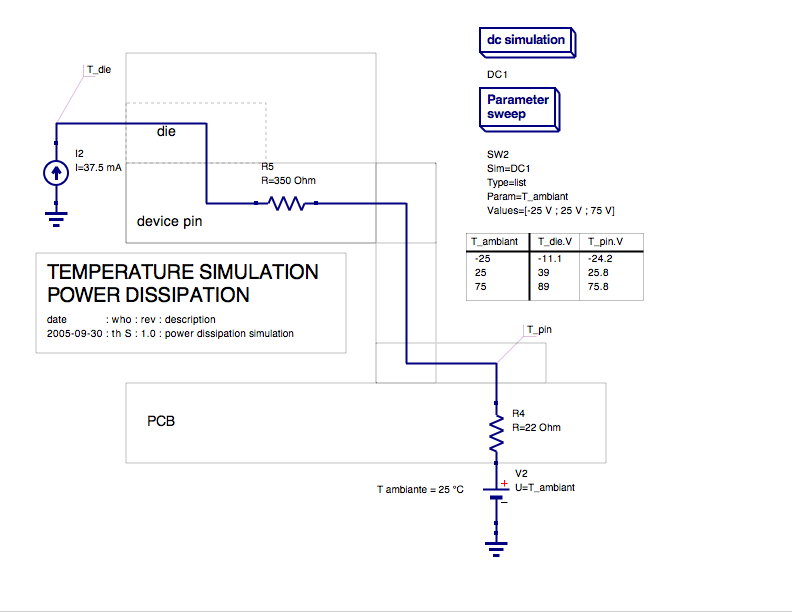
\includegraphics[scale=0.5]{powerDissipation}
	\caption{Schematics used to simulate the DC power dissipation}
	\label{design:pa:bias:DCpower}
\end{center}
\end{figure}


\tutsection{Small signal analysis}

The current version of QUCS do not include an Harmonic Balance solver, so we need to do some other simualtions in order to have some ideas on the performances of our design.
